\documentclass{article}
\usepackage[utf8]{inputenc}
\usepackage{graphicx}
\usepackage{hyperref}
\usepackage{amsmath}


\usepackage{tikz}
\usetikzlibrary{positioning, arrows}


\usepackage{stackengine,amssymb,graphicx}
\newcommand\DDiamond{\ensurestackMath{%
  \stackengine{.5pt}{\Diamond}{\scalebox{.75}[1]{$-$}}{O}{c}{F}{F}{L}}}

  \newcommand{\sol}{\textbf{solution}}

\title{CSE105/209A: Modern Algorithmic Toolbox\footnote{PI: Vaggos Chatziafratis}, PSET-3,\\ \textbf{Deadline:} \textbf{7 days from now}}
\author{Ian Chi}
\date{}
\begin{document}
\maketitle
% \vspace{-2cm}
\paragraph{Instructions:} Deadline in \textbf{7 days, 11:59pm}. Submit to Canvas a pdf of your solutions, with your name and ucsc id number. Feel free to discuss solutions with your colleagues (other students), explore the internet, read and be inspired from the textbooks etc. But what you type should be typed by you and you only in latex. In algorithms, we appreciate brevity and accuracy: your solutions should be to the point, often one or two sentences suffice to provide all necessary details and descriptions. Unnecessarily long answers will not get full credit.\\




\noindent \textbf{Ex.1 (30pts) (Review of Linear Algebra)}

Just to review some basic concepts from linear algebra we ask you to prove the following (if referenced, matrix $A$ is real and symmetric):

\begin{enumerate}
    \item Prove: If $A$ is a real, symmetric $n \times n$ matrix, then all of its eigenvalues are real.
    
    \sol 
    consider the sesquilinear  form 
    \begin{equation}
        \langle .,A.\rangle
    \end{equation}

    if we now coinsider 

    \begin{equation}
        \langle v,Av\rangle 
    \end{equation}
    where \(v\) is an eigenvector of A,

    \begin{equation}
        \begin{split}
        \lambda \langle v,v\rangle &= \langle v,Av\rangle\\
        &= \langle \bar A v,v\rangle \\
        &= \bar \lambda\langle  v,v\rangle 
        \end{split}
    \end{equation}

    thus \(\bar \lambda = \lambda\) which implies lambda is real. 



    \item Let $\lambda_i$ and $\lambda_j$ be two eigenvalues of a symmetric matrix $A$, and $u_i$, $u_j$ be the corresponding eigenvectors. Prove the following: If $\lambda_i \neq \lambda_j$, then
$u_i^Tu_j  = 0$ (inner product is zero so vectors are orthogonal).

\sol

    \begin{equation}
        \lambda_i\langle u_i, u_j\rangle =\langle Au_i, u_j\rangle =\langle u_i, A u_j\rangle = \lambda_j\langle u_i, u_j\rangle 
    \end{equation}
    which can only hold if \(\langle u_i,u_j\rangle\) is zero since \(\lambda_i,\neq \lambda_j\)
    \item More generally, it is without loss of generality that we can assume that the eigenvectors of $A$ form an orthonormal basis for $\mathbb{R}^n$ (recall, orthonormal basis is a set of vectors that are all of unit length, and any two of them are orthogonal to each other, for example the standard basis vectors form an orthonormal basis).
    
    

    
    Prove:  Let $\lambda_1 \le\ldots \le  \lambda_n$ be the eigenvalues of $A$ with corresponding eigenvectors $u_1,\ldots,u_n$. Then, $A = \sum_{i=1}^n \lambda_iu_iu_i^T$ (note this $u_iu_i^T$ is \textbf{not} the inner product of the vectors and the result is a matrix).

    \sol 

    since the eigenvectors form an orthonormal basis we can represent any vector \(v\) as \(v=\sum c_i  u_i\) where \(u_i\) are the orthonormal eigenbasis vectors. since we know how each one scales, we can represent each \(u_i\) acted on by \(A\) as \(\lambda_i u_i u_i^T c_i u_i = c_i\lambda_i u_i\). doing this term by term in our decomposition of \(v\) shows that \(A\) is indeed 
    \(\sum_{i=1}^n \lambda_iu_iu_i^T\)
    \item Prove the following characterization for the largest eigenvalue (analogous characterizations hold for all other eigenvalues): If $A$ is an $n \times n$ real symmetric matrix, then the largest eigenvalue of $A$ is
    \[
    \lambda_n(A) = \max_{v\in \mathbb{R}^n\setminus\{0\}} \frac{v^TAv}{v^Tv}
    \]
    (Hint: use the fact from part 3 that the eigenvectors form an orthonormal basis to express any vector $v$...)

    \sol

    for any normalized vector \(v\), we can see the equation is actually just 
    
    \begin{equation}
        \lambda_n(A) = \max_{v\in \mathbb{R}^n\setminus\{0\}} \frac{v^TAv}{v^Tv} = \max_{v\in \mathbb{R}^n\setminus\{0\}} \frac{v^TAv}{1} 
    \end{equation}
    so we shall work with normalized vectors instead. any normalized vector can be written as linear combination of eigenbasis, so we can write the term as 
    \begin{equation}
        \begin{split}
            \lambda_n(A) &= \max_{v\in \mathbb{R}^n\setminus\{0\}} \left(\sum c_i w_i\right)^TA \left(\sum c_i w_i\right) \\
            &= \max_{v\in \mathbb{R}^n\setminus\{0\}} \left(\sum c_i w_i\right)^T \left(\sum \lambda_i c_i w_i\right)\\
            &= \max_{v\in \mathbb{R}^n\setminus\{0\}} \sum c_i \sum \lambda_j c_j\delta_{ij}\\
        \end{split}
    \end{equation}

    where \(\delta_{ij}\) is the kronecker delta,

    note that since the vectors are normalized, the squared sum of \(c_i\) is also normalized. the way to get the largest value is therefore for \(c_L=1\) for \(L\) corresponding to the index of the largest eigenvector 



    \item Using part 4, prove that for any unweighted, undirected graph the largest eigenvalue of its Laplacian $L$ is at least the maximum degree of the graph $G$, in other words prove:
    \[
    \lambda_{max}(L)\ge d_{max}(G)
    \]
    (Hint: as always the quadratic form of the Laplacian should be used)
    \textbf{Bonus/Grads:} Show that actually we can do slightly better: $\lambda_{max}(L)\ge d_{max}(G)+1$. 


    \sol 

    consider the vector \(d_{max}\) is on the vertex with the highest degree, \(-1\) on all elements adjacent to the vertex a value of -1, and 0 on all other vertecies. we should notice that every edge contributes \((d_{max}+1)^2\) to \(xLx\) and there are \(d_max\) edges. 

    the norm of this vector comes out to be \(d_{max}(d_{max}+1)\) and thus the largest eigenvalue, which is always \(\geq\) the quadratic form for any vector, must be greater than or equal to \(d_{max}+1\)
    


    \item Let $P_n$ be the path graph on $n$ nodes. Prove that $\lambda_2(P_n) = O(\frac{1}{n^2})$.
    
    (Hint: Here you should use the characterization for the second smallest eigenvalue of the Laplacian: $\lambda_2(L)=\min_{v\in \mathbb{R}^n\setminus\{0\},v^T\cdot \textbf{1}=0} \frac{v^TAv}{v^Tv}$, where $\textbf{1}$ is the all-1s vector... One more hint: maybe the vector whose $i^{th}$ coordinate is $n+1-2i$ will be helpful in the proof.)\\

    \sol
    if we can find a single vector that has a quadratic form value that is \(O(\frac{1}{n^2})\), then the second eigenvalue must be \(\leq\) that vectors quadratic form value. 

    consider the vector described in the hint. 

    \begin{equation}\begin{split}
            \frac{x^TLx}{x^Tx} &= \frac{n-1}{\sum (n+1-2i)^2}\\
    \end{split}
    \end{equation}

    but notice the denominator is approximately \(O(\sum_0^n n^2) = O(n^3)\)
    which means the whole expression is \(O(\frac{1}{n^2})\)

    so thus the second eigenvalue must be \(O(\frac{1}{n^2})\).


\end{enumerate}







\newpage
\noindent \textbf{Ex.2 (20pts) (Two More Motifs)}
See Figure 1 that shows two more motif equations like the previous homeworks. Here, we use the adjacency matrix $A$  and also the adjacency matrix $C$ of the complement graph. We ask you to prove the two motif equations. ($P_4$: this is the path on 4 nodes, and the other patterns are as shown in the figure.)\\



\begin{figure}[ht]
    \centering
    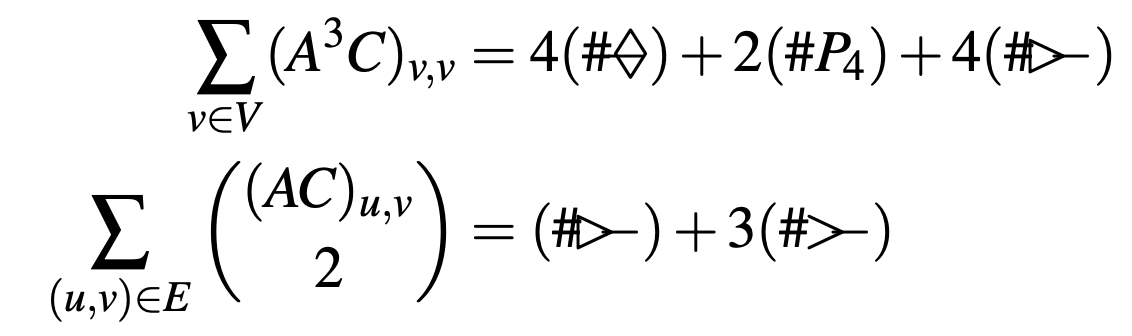
\includegraphics[width=9cm]{Screen Shot 2025-04-25 at 22.44.12.png}
    \caption{Two extra Motif Equations. The matrix $C$ corresponds to the complement graph.}
    \label{fig:my_label}
\end{figure}

\sol 

let us draw out all the possible ways the path is counted for each of the motifs in equation 1. let the red line represent no edge and the black lines represent edges
\begin{enumerate}
    \item 
    In a diamond, there are 4 ways to travel along 1 edge then 3 edges to return to the original vertex.
    
    
    \begin{figure}[!ht]
    \centering
    \resizebox{0.5\textwidth}{!}{%
    \begin{tikzpicture}
    \tikzstyle{every node}=[font=\fontsize{18.2pt}{23.7pt}\selectfont]
    
    \draw [] (8.375,13.25) -- (6.75,11.25);
    \draw [] (6.875,11.25) -- (9,11.125);
    \draw [] (9.125,11.125) -- (8,9.125);
    \draw [ color={rgb,255:red,255; green,0; blue,0}, draw opacity=1, ] (8,9.125) -- (8.375,13.25);
    \draw [ color={rgb,255:red,255; green,0; blue,0}, draw opacity=1, ] (11.875,12.75) -- (11.5,9.25);
    \draw [] (11.875,12.625) -- (12.75,10.75);
    \draw [] (12.75,10.75) -- (10.625,11);
    \draw [] (10.5,10.875) -- (11.5,9.25);
    \node [font=\fontsize{18.2pt}{23.7pt}\selectfont, inner xsep=0.080cm, inner ysep=0.085cm, rounded corners=0.020cm] at (8.375,13.75) {a};
    \node [font=\fontsize{18.2pt}{23.7pt}\selectfont, inner xsep=0.080cm, inner ysep=0.085cm, rounded corners=0.020cm] at (7.75,8.875) {b};
    \node [font=\fontsize{18.2pt}{23.7pt}\selectfont, inner xsep=0.080cm, inner ysep=0.085cm, rounded corners=0.020cm] at (11.625,13.375) {c};
    \node [font=\fontsize{18.2pt}{23.7pt}\selectfont, inner xsep=0.080cm, inner ysep=0.085cm, rounded corners=0.020cm] at (11.625,8.375) {d};
    \end{tikzpicture}
    
    }%
    
    \caption{Four ways to count diamond, starting at nodes \(a,b,c,d\)}
    \label{fig:diamond_1}
    \end{figure}
    
    
    \begin{figure}[!ht]
    \centering
    \resizebox{0.5\textwidth}{!}{%
    \begin{tikzpicture}
    \tikzstyle{every node}=[font=\fontsize{18.2pt}{23.7pt}\selectfont]
    \draw [] (6.125,12.125) -- (8,13.625);
    \draw [] (8,13.625) -- (10.5,13.625);
    \draw [] (10.5,13.625) -- (11.75,12.375);
    \draw [ color={rgb,255:red,255; green,0; blue,0}, draw opacity=1, ] (11.625,12.5) -- (6.25,12.25);
    \node [font=\fontsize{18.2pt}{23.7pt}\selectfont, inner xsep=0.080cm, inner ysep=0.085cm, rounded corners=0.020cm] at (5.875,11.875) {a};
    \node [font=\fontsize{18.2pt}{23.7pt}\selectfont, inner xsep=0.080cm, inner ysep=0.085cm, rounded corners=0.020cm] at (11.75,11.875) {b};
    \end{tikzpicture}
    }%
    \caption{two ways to count the four path, staring at \(a,b\)}
    \label{fig:path_1}
    \end{figure}
    
    \begin{figure}[!ht]
    \centering
    \resizebox{0.9\textwidth}{!}{%
    \begin{tikzpicture}
    \tikzstyle{every node}=[font=\fontsize{18.2pt}{23.7pt}\selectfont]
    \draw [ color={rgb,255:red,255; green,0; blue,0}, draw opacity=1, ] (6.125,10.25) -- (10.5,11.75);
    \draw [ color={rgb,255:red,255; green,0; blue,0}, draw opacity=1, ] (16.75,12.875) -- (20.75,11.375);
    \draw [] (10.375,11.75) -- (8,11.625);
    \draw [] (8,11.75) -- (6.25,12.625);
    \draw [] (6.25,12.625) -- (6.125,10.375);
    \draw [] (20.5,11.375) -- (18.25,11.25);
    \draw [] (18.25,11.25) -- (16.75,10.625);
    \draw [] (16.75,10.625) -- (16.75,12.75);
    \node [font=\fontsize{18.2pt}{23.7pt}\selectfont, inner xsep=0.080cm, inner ysep=0.085cm, rounded corners=0.020cm] at (10.75,12) {a};
    \node [font=\fontsize{18.2pt}{23.7pt}\selectfont, inner xsep=0.080cm, inner ysep=0.085cm, rounded corners=0.020cm] at (6,9.75) {b};
    \node [font=\fontsize{18.2pt}{23.7pt}\selectfont, inner xsep=0.080cm, inner ysep=0.085cm, rounded corners=0.020cm] at (16.25,13) {c};
    \node [font=\fontsize{18.2pt}{23.7pt}\selectfont, inner xsep=0.080cm, inner ysep=0.085cm, rounded corners=0.020cm] at (21.125,11.25) {d};
    \end{tikzpicture}
    }%
    \caption{four ways to count tailed triangle starting at \(a,b,c,d\)}
    \label{fig:tt_1}
    \end{figure}

    \newpage
    \item 

    this motif counts: how many combinations of two are there to go from \(u\) to \(v\) given one non edge to one edge AND there being an edge from \(u\) to \(v\). 


    in the tailed triangle, there are exactly two ways for this to happen

    notice in figure~\ref{fig:tt_2}, there are exactly two paths of length two, crosing one non edge (dashed), then 1 edge (solid) going from \(v\) to \(u\). There are no other ways for this motif to be counted in the equation.

    \begin{figure}[!ht]
\centering
\resizebox{0.5\textwidth}{!}{%
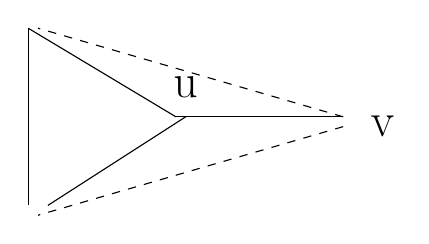
\begin{tikzpicture}
\tikzstyle{every node}=[font=\fontsize{18.2pt}{23.7pt}\selectfont]
\draw  (7.5,12.25) -- (7.5,10);
\draw  (7.5,12.25) -- (9.375,11.125);
\draw  (7.75,10) -- (9.5,11.125);
\draw  (9.375,11.125) -- (11.5,11.125);
\node [font=\fontsize{18.2pt}{23.7pt}\selectfont, inner xsep=0.080cm, inner ysep=0.085cm, rounded corners=0.020cm] at (9.5,11.5) {u};
\node [font=\fontsize{18.2pt}{23.7pt}\selectfont, inner xsep=0.080cm, inner ysep=0.085cm, rounded corners=0.020cm] at (12,11) {v};
\draw [dashed] (11.5,11.125) -- (7.625,12.25);
\draw [dashed] (11.5,11) -- (7.625,9.875);
\end{tikzpicture}
}%
\caption{tailed triangle motif}
\label{fig:tt_2}
\end{figure}


in the 4 star graph there are 3 ways to choose two. where in the tailed triangle only 1 edge was a candidate \((u,v)\), all three edges have two paths in the same way figure~\ref{fig:tt_2} depicts thus a 4 star graph is counted 3 times. 


\end{enumerate}






\newpage

\noindent \textbf{Ex.3 (20pts) (Embedding the Petersen graph)} 
Check Figure 2 where we show the Petersen graph. We ask you the following:
\begin{itemize}
    \item Compute the eigenvalues and eigenvectors of the Laplacian $L$ matrix. Please comment on the symmetry observed.

    

    \item Do the spectral embedding of the Petersen graph onto the second and third smallest eigenvectors of $L$.
    \item Compute the second eigenvector and run the sweeping cut algorithm to split the graph into two pieces $S$ and $V\setminus S$, so as to (try to) minimize the isoperimetric ratio. Output the set $S$, its boundary and its isoperimetric ratio. What is the optimum isoperimetric ratio of the graph?
    \item Choose any vertex that you want and delete two of its edges. Then repeat parts 1,2,3 for this graph.
\end{itemize}

\begin{figure}[ht]
    \centering
    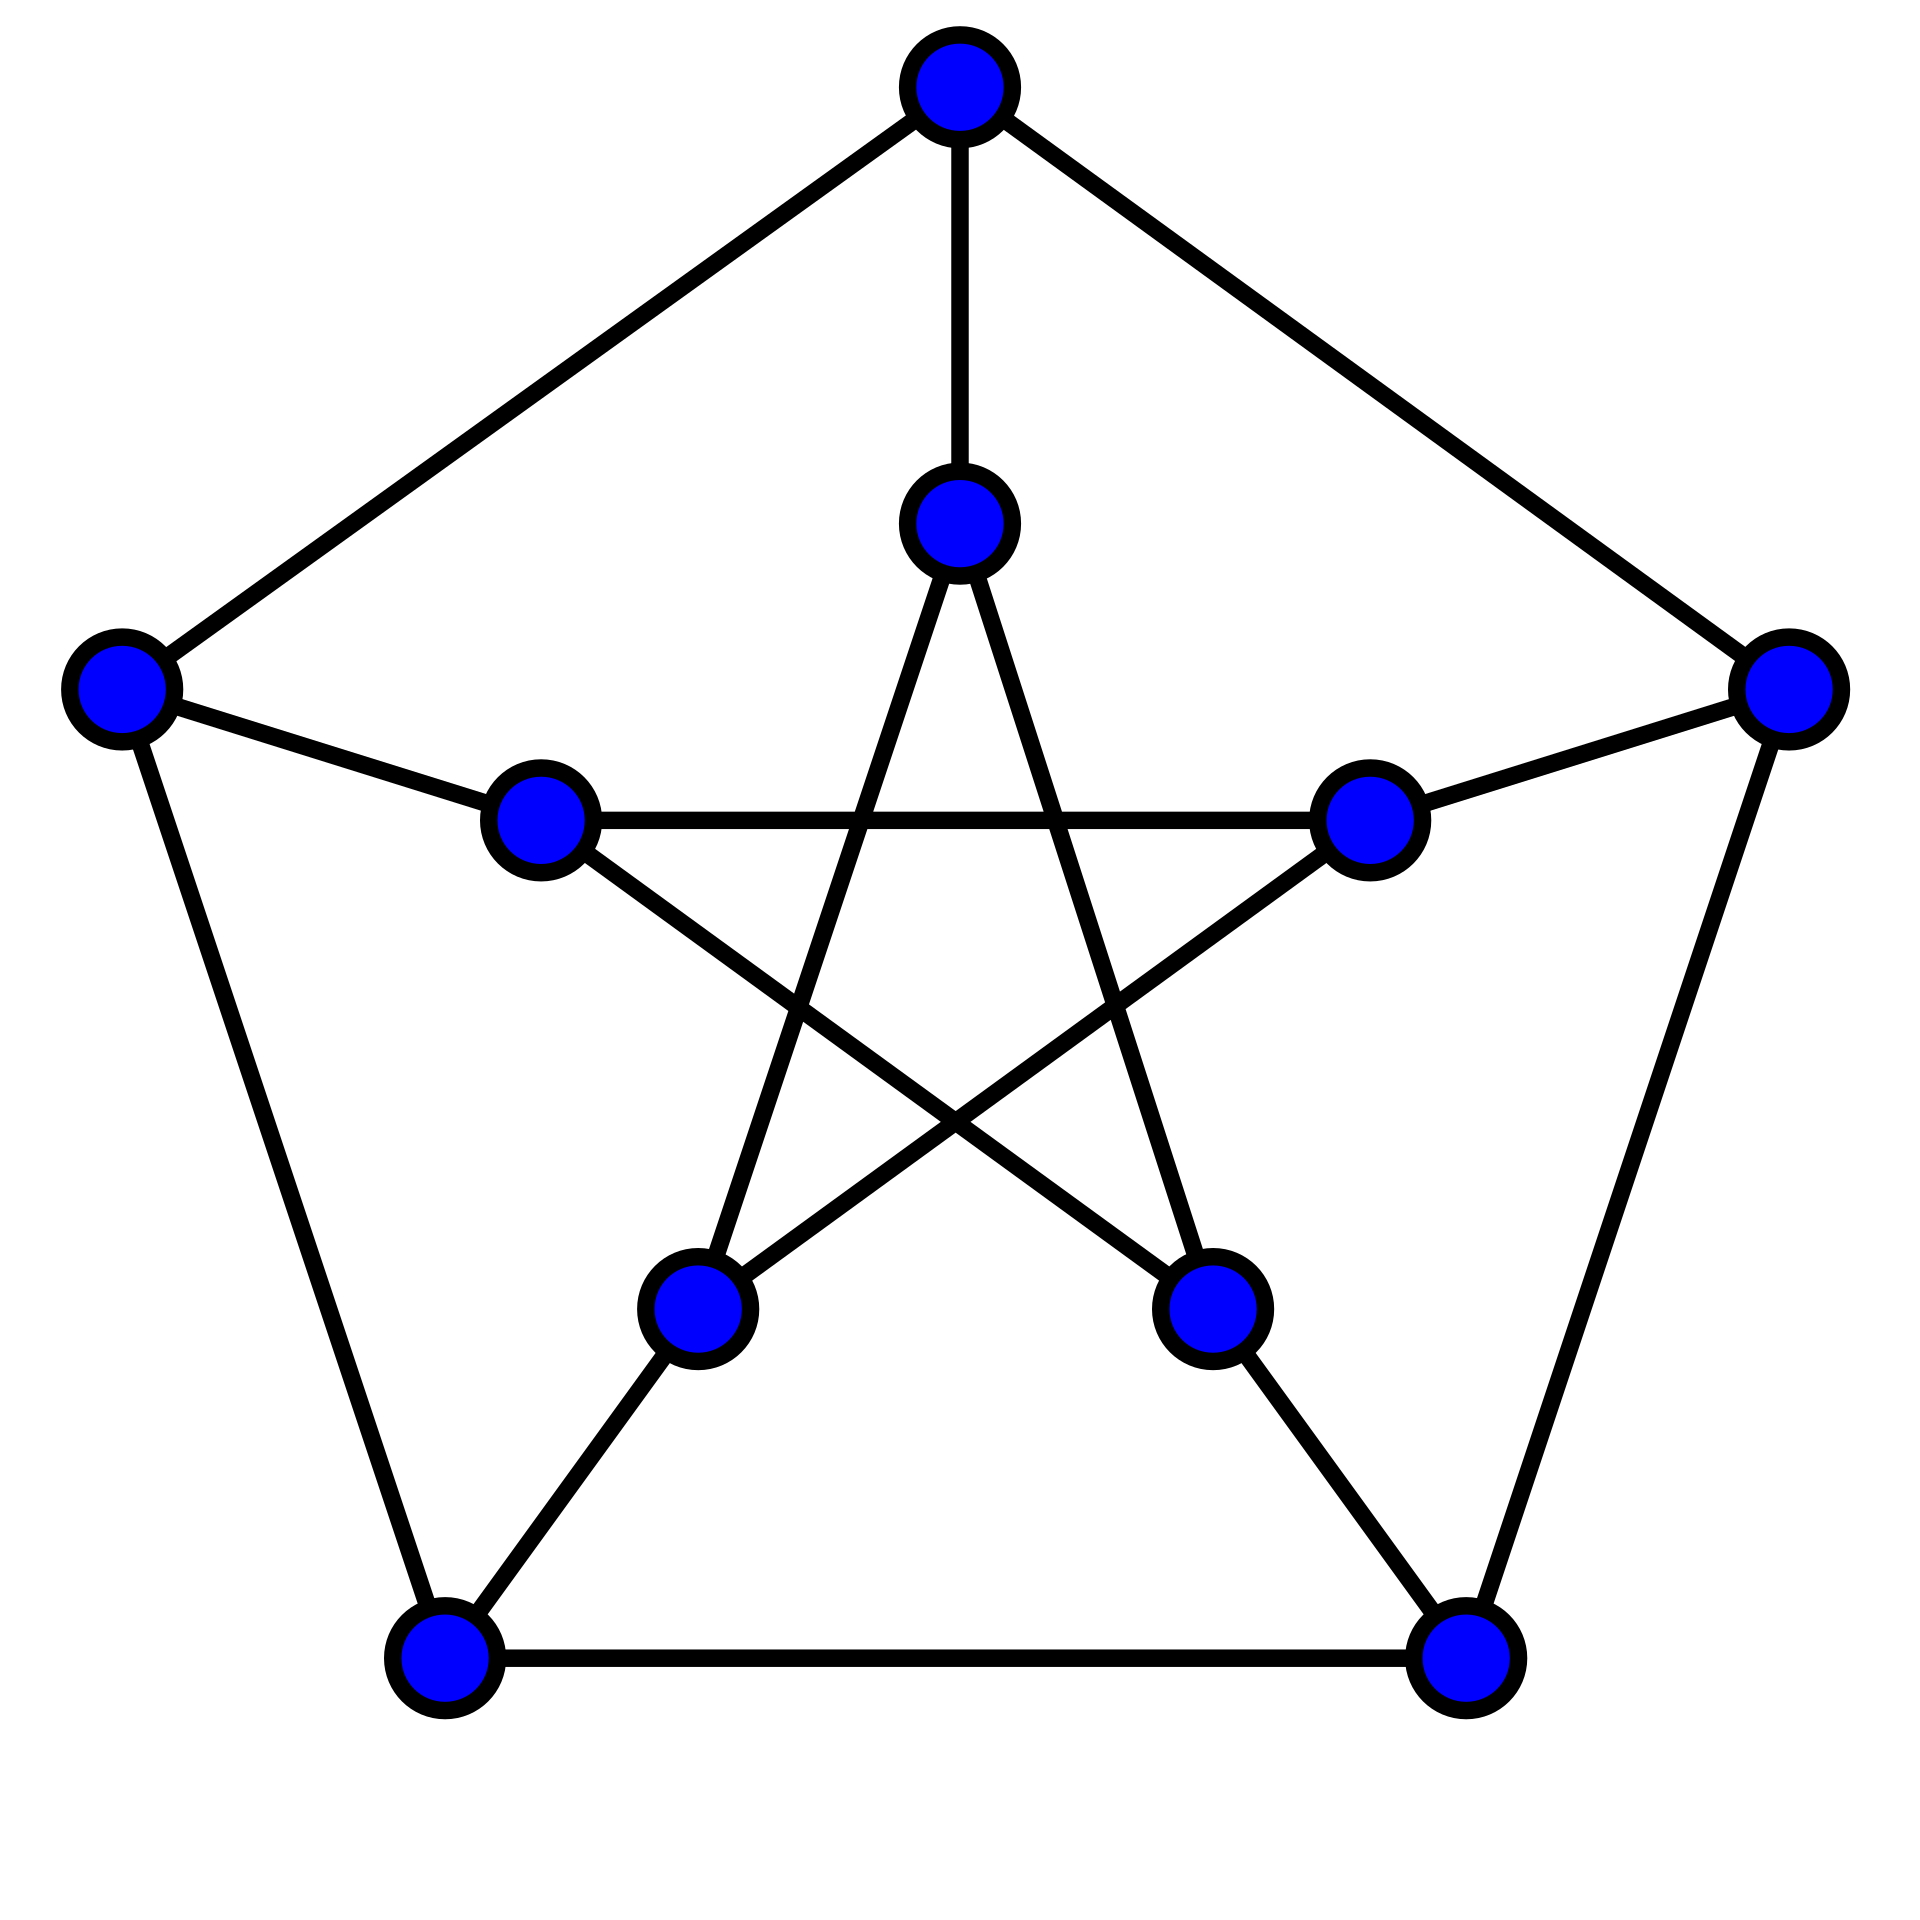
\includegraphics[width=6cm]{Petersen1_tiny.svg.png}
    \caption{The Petersen Graph.}
    \label{fig:my_label}
\end{figure}

\newpage
\noindent \textbf{Ex.4 (30pts) (Interview Question I: Geometry and Embeddings)}

Here we explore embeddings of random points. (feel free to use any software/programming language you want to do the calculations (e.g., Python or Matlab) and you don't have to include your calculations, just your final answers and plots.)


\begin{itemize}
    \item Pick 100 random points in the unit square, by independently choosing their $x$ and $y$ coordinates uniformly at random from the interval [0,1] (there are many Python implementations for this). Form a graph by adding an edge between every pair of points whose Euclidean distance is at most $\frac{1}{4}$. 

Using the Laplacian, plot the embedding of the graph onto the second and third eigenvectors (those that correspond to the second and third smallest eigenvalues). Here do \textbf{not} overlay the edges of the graph just plot the vertices.

\item Now, for all points in the original dataset whose $x$ and $y$ coordinates are \textbf{both less} than $\frac 12$, plot their images in the embedding in a different color. Are these points clustered together in the embedding? Why does this make sense?\\
\end{itemize}





\end{document}

